\newpage
\section{Data and Monte Carlo samples}
\label{sec:data_and_mc_samples1}


The data sample of proton-proton collisions at $\sqrt{s}=8$~\TeVcc was collected in 2012 and corresponds to
an integrated luminosity of \intlumi.
The datasets and also the certifications
used are summarized in Table~\ref{table:dataset}. 
The certification file used for these data is 
{\tt Cert\_190456-208686\_8TeV\_22Jan2013ReReco\_Collisions12\_JSON.txt
}. The dijet sample is dominated by light flavored and gluon jets, which we denote as 
the ``QCD background".  The QCD background is obtained from data by fitting an
analytic parameterization of the dijet invariant mass distribution.

\begin{table}[!htb]
\begin{center}
\begin{tabular}{c}
\hline
Dataset                                 \\
\hline
/Jet/Run2012A-22Jan2013-v1/AOD  \\
/JetHT/Run2012B-22Jan2013-v1/AOD  \\
/JetHT/Run2012C-22Jan2013-v1/AOD  \\
/JetHT/Run2012D-22Jan2013-v1/AOD  \\
\hline
\end{tabular} 
\end{center}
\caption{Summary of 8\TeVcc collision data used in this analysis. 
}
\label{table:dataset}
\end{table}



Signal events have been simulated using
{\sc jhugen}~\cite{Gao:2010qx,Bolognesi:2012mm},
\PYTHIA~6.426~\cite{pythia} and \HERWIG{++} 2.5.0~\cite{herwig} event
generators and processed through a simulation of the CMS detector,
based on \GEANTfour~\cite{refGEANT}.  \PYTHIA~6 is used with
CTEQ6L1~\cite{cteq} and \HERWIG{++} with MRST2001~\cite{mrst} parton
distribution functions.  Tune Z2* (a modification of tune
Z1~\cite{bib_tunez1}) is used with \PYTHIA~6, while the tune version
23 is used with \HERWIG{++}.  The process $\cPq^* \to \PW/\cPZ +
\text{jet}$ is generated using \PYTHIA~6.  RS graviton production is
studied with $k/\MPl=0.1$, which determines a resonance width of about
1\% of the resonance mass which is about a factor five smaller than
the experimental resolution for dijets.  While \HERWIG{++} contains a
more detailed description of the angular distributions for \GRS than
\PYTHIA~6 for this process~\cite{resonanceshape} and is therefore used
to model the \GRS resonance shape, the \PYTHIA~6 cross section is used
to maintain consistency with reference models used in related
analyses~\cite{CMSZZPAS2}.  Bulk graviton production is studied with
$k/\MPl=0.2$ and is generated with {\sc jhugen} interfaced with
\PYTHIA~6 for the showering.
Bulk graviton cross sections are calculated using CalcHEP.
The process $\PWpr \to \PW\cPZ$ is generated using \PYTHIA~6 with Standard
Model $V-A$ couplings and without applying k-factors.  

To validate our RS graviton resonance Monte Carlo, we compare \PYTHIA~6, \HERWIG{++} and 
a generator including full angular correlations developed by the JHU group (which
we denote ``JHU generator'').
Figure~\ref{fig:compare-Herwig++-Pythia6} shows the comparsions of invariant mass and
$\Delta\eta$ of two Z bosons at generator level, in which \HERWIG{++} and
\PYTHIA~6 are compared with the JHU generator which describes the
angular distributions exactly.  \PYTHIA~6 does not implement the angular
correlations, and from Figure~\ref{fig:compare-Herwig++-Pythia6} one can indeed conclude
that in its description of this effect it is inferior to \HERWIG{++}.

\begin{figure}[htb]
\begin{center}
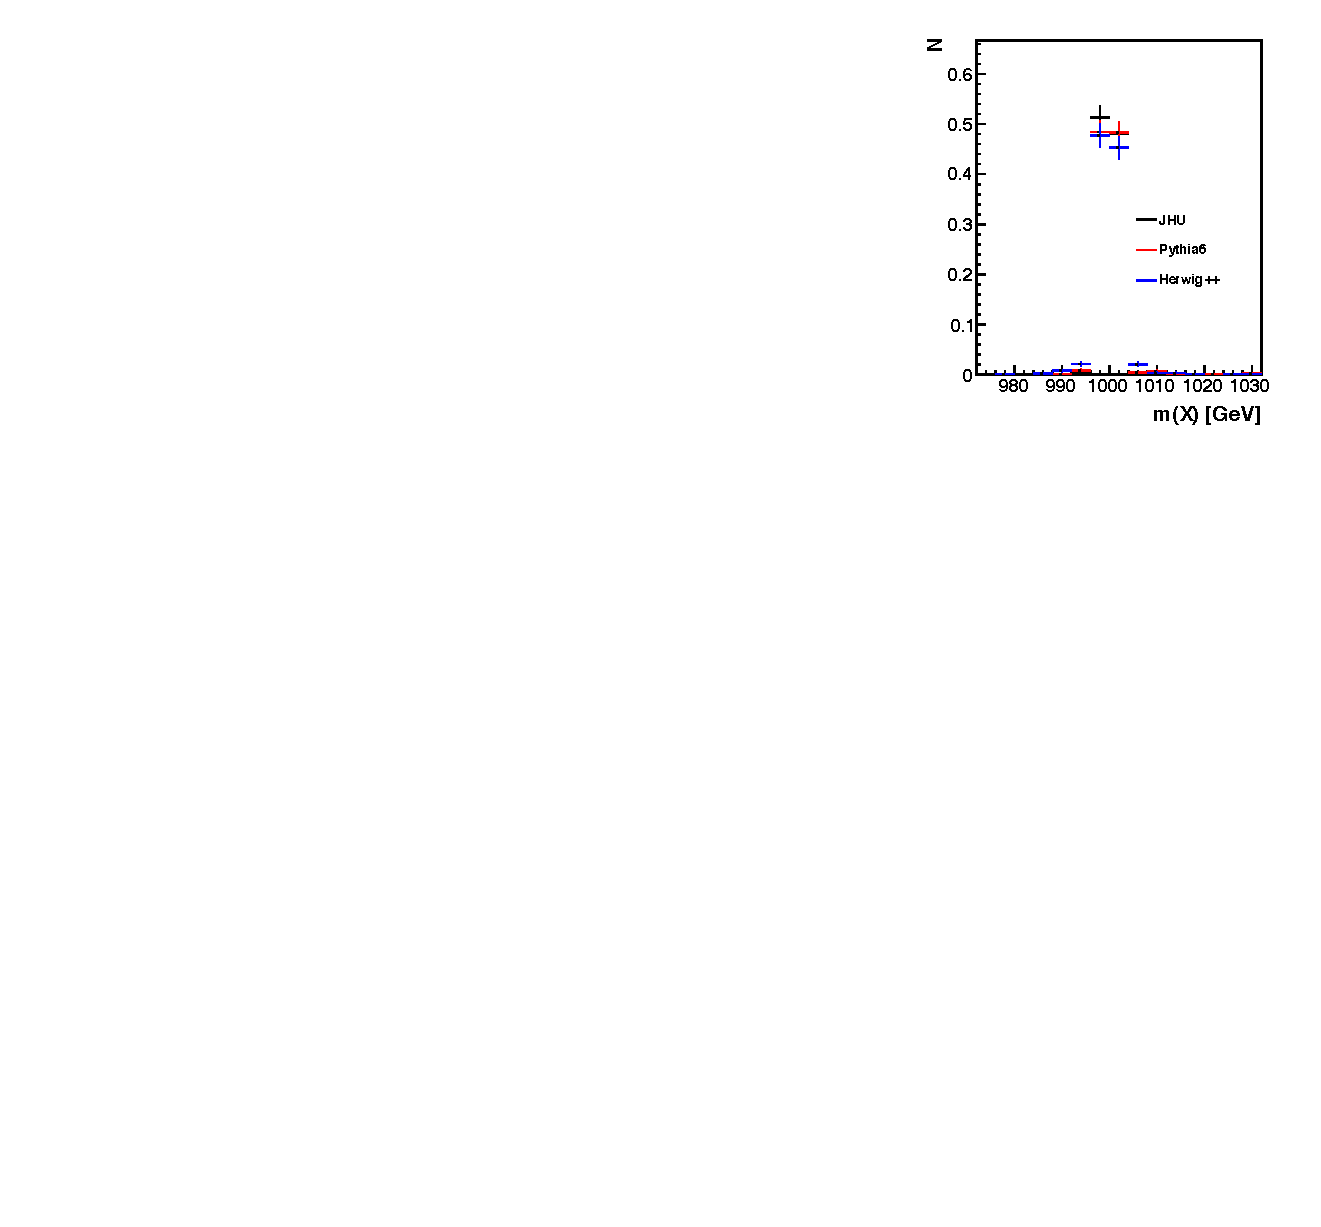
\includegraphics[width=0.43\textwidth]{EXO-12-024/figs/comparison-jhu-pythia-herwigg/MX.pdf}
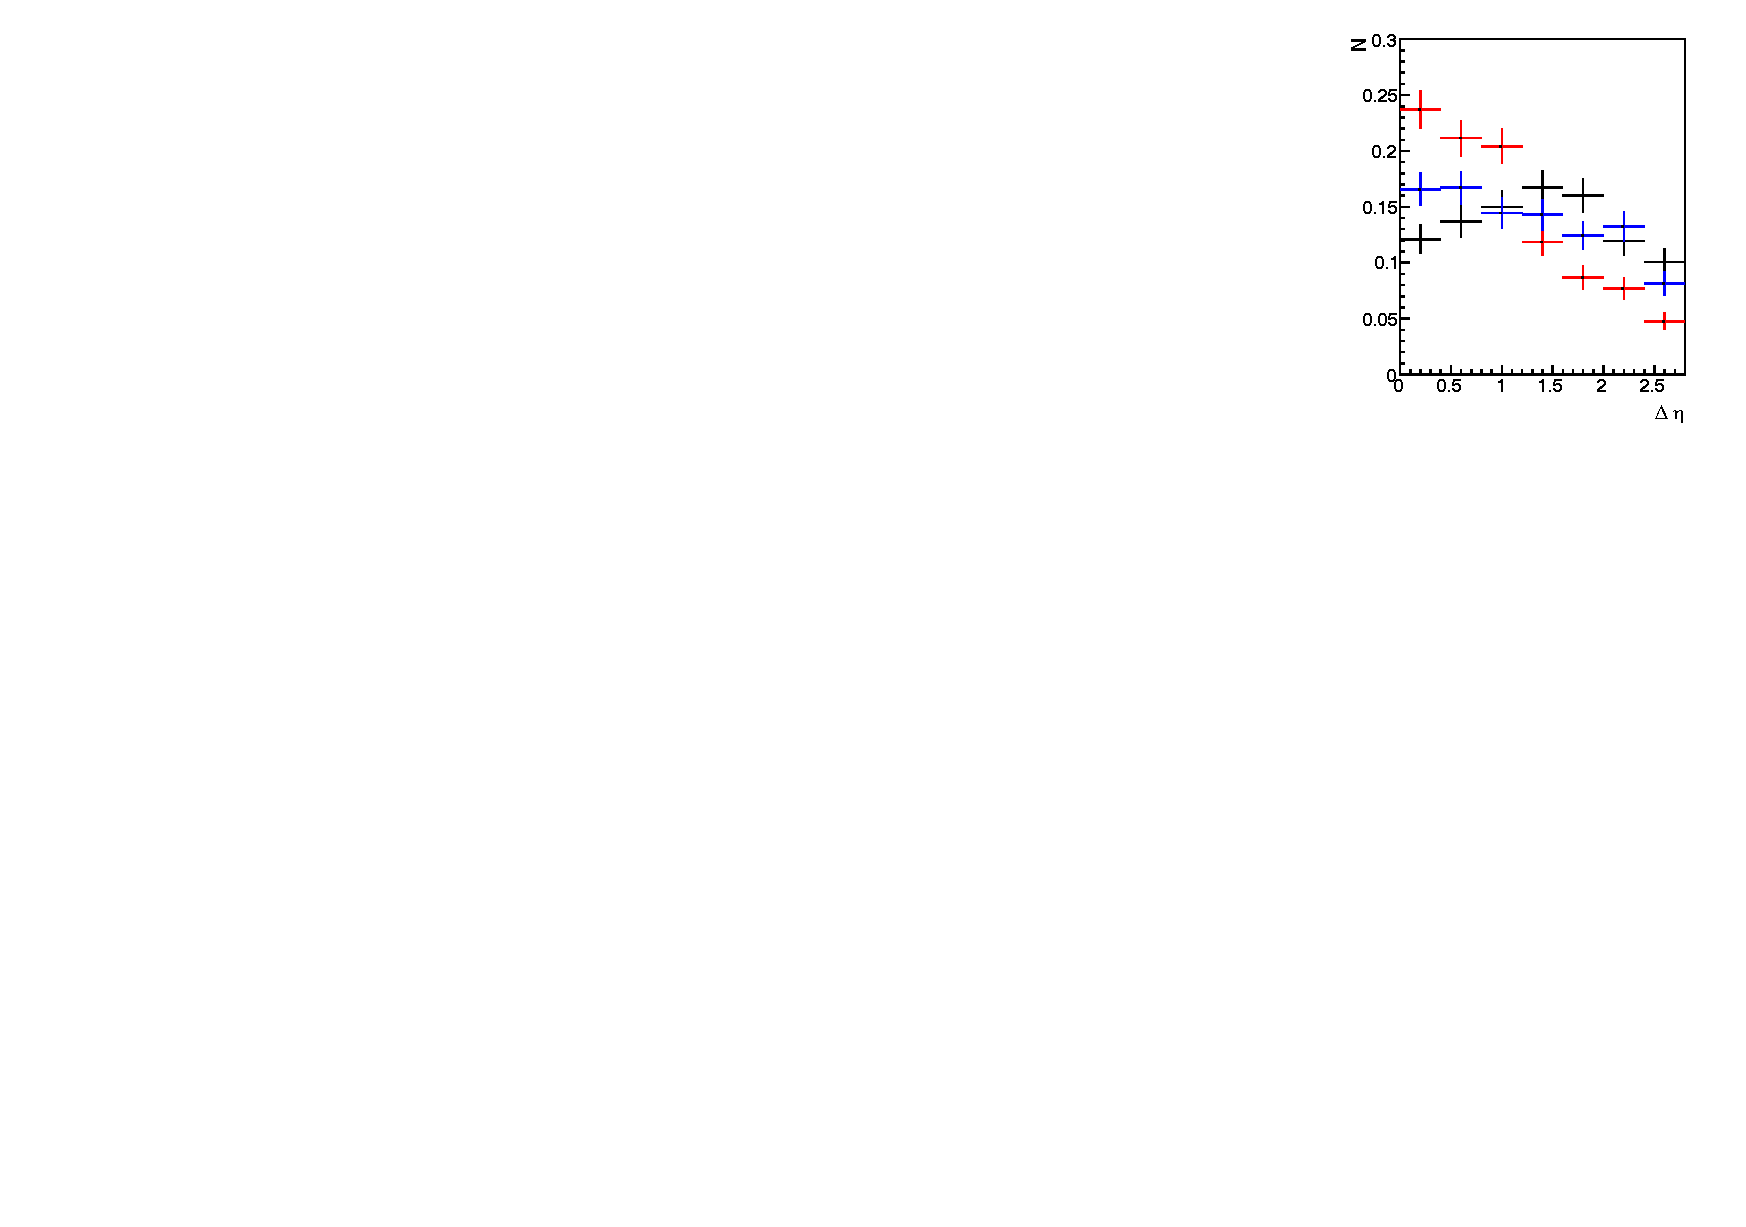
\includegraphics[width=0.43\textwidth]{EXO-12-024/figs/comparison-jhu-pythia-herwigg/delta-y.pdf}
\end{center}
\caption{Invariant mass and $\Delta\eta$ of two Z bosons at generator level for Pythia6 and Herwig++ models of a 1~\TeVcc RS graviton resonance with $k/M_{PL}=0.02$ with the JHU generator which includes all angular correlations.}
\label{fig:compare-Herwig++-Pythia6}
\end{figure}

All Monte Carlo events are fully simulated and reconstructed via the Geant4-based CMS simulation
 and reconstruction software.

Tables~\ref{table:singletag}, \ref{table:doubletag}, \ref{table:doubletagbulk} and \ref{table:doubletag2} summarize the new 
physics simulation datasets used in this analysis. 




\begin{table}[htb]
\begin{center}
\begin{tabular}{ cccc }
\hline
Process           & Generator& Events & X-sec[pb] \\
\hline
qW(m=750\GeVcc) &Pythia6   &30000   &1.133E+02  \\
qW(m=1000\GeVcc)&Pythia6   &30000   &2.647E+01  \\
qW(m=1500\GeVcc)&Pythia6   &30000   &2.540E+00  \\
qW(m=2000\GeVcc)&Pythia6   &30000   &3.510E-01  \\
qW(m=3000\GeVcc)&Pythia6   &30000   &1.008E-02  \\

qZ(m=750\GeVcc) &Pythia6   &30000   &4.071E+01  \\
qZ(m=1000\GeVcc)&Pythia6   &30000   &9.405E+00  \\
qZ(m=1500\GeVcc)&Pythia6   &30000   &8.937E-01  \\
qZ(m=2000\GeVcc)&Pythia6   &30000   &1.231E-01  \\
qZ(m=3000\GeVcc)&Pythia6   &30000   &3.465E-03  \\
\hline
\end{tabular}
\end{center}
\caption{Summary of the simulated Monte Carlo samples used in this analysis for process
 ${\rm q* \to Z/W + jet}$}
\label{table:singletag}
\end{table}


\begin{table}[htb]
\begin{center}
\begin{tabular}{ cccc }
\hline
Process            & Generator             & Events& Pythia6 x-sec [pb] \\
\hline
WW(m=750\GeVcc)  &Herwig++/Pythia6 Z2*   &30000  & 2.220E+00\\
WW(m=1000\GeVcc) &Herwig++/Pythia6 Z2*   &30000  & 4.254E-01 \\
WW(m=1500\GeVcc) &Herwig++/Pythia6 Z2*   &30000  & 3.298E-02 \\
WW(m=2000\GeVcc) &Herwig++/Pythia6 Z2*   &30000  & 4.083E-03 \\
WW(m=2500\GeVcc) &Herwig++/Pythia6 Z2*   &30000  & 6.191E-03 \\
WW(m=3000\GeVcc) &Herwig++/Pythia6 Z2*   &30000  & 1.010E-04 \\
ZZ(m=750\GeVcc)  &Herwig++/Pythia6 Z2*   &30000  & 1.120E+00 \\
ZZ(m=1000\GeVcc) &Herwig++/Pythia6 Z2*   &30000  & 2.137E-01 \\
ZZ(m=1500\GeVcc) &Herwig++/Pythia6 Z2*   &30000  & 1.662E-02 \\
ZZ(m=2000\GeVcc) &Herwig++/Pythia6 Z2*   &30000  & 2.027E-03 \\
ZZ(m=2500\GeVcc) &Herwig++/Pythia6 Z2*   &30000  & 3.077E-04 \\
ZZ(m=3000\GeVcc) &Herwig++/Pythia6 Z2*   &30000  & 5.099E-05 \\
\hline
\end{tabular}
\end{center}
\caption{Summary of the simulated Monte Carlo samples used in this analysis for process
 ${\rm G_{RS} \to WW, ZZ}$.}
\label{table:doubletag}
\end{table}

\begin{table}[htb]
\begin{center}
\begin{tabular}{ cccc }
\hline
Process           & Generator& Events & X-sec[pb] \\
\hline
WZ(m=750\GeVcc) &Pythia6   &30000   &5.391E-01  \\
WZ(m=1000\GeVcc)&Pythia6   &30000   &1.444E-01 \\
WZ(m=1500\GeVcc)&Pythia6   &30000   &1.804E-02  \\
WZ(m=2000\GeVcc)&Pythia6   &30000   &3.129E-03  \\
WZ(m=2500\GeVcc)&Pythia6   &30000   &6.781E-04  \\
WZ(m=3000\GeVcc)&Pythia6   &30000   &1.894E-04  \\
\hline
\end{tabular}
\end{center}
\caption{Summary of the simulated Monte Carlo samples used in this analysis for process
 ${\rm W' \to WZ}$.}
\label{table:doubletag2}
\end{table}


\begin{table}[htb]
\begin{center}
\begin{tabular}{ cccc }
\hline
Process            & Generator             & Events & X-sec[pb] \\
\hline
WW(m=1000\GeVcc) &JHU Z2*   &50000  &0.001774 \\
WW(m=1500\GeVcc) &JHU Z2*   &50000  &9.207E-05 \\
WW(m=2000\GeVcc) &JHU Z2*   &50000  &8.004E-06 \\
WW(m=2500\GeVcc) &JHU Z2*   &50000  &8.851E-07 \\
WW(m=3000\GeVcc) &JHU Z2*   &50000  &- \\
ZZ(m=1000\GeVcc) &JHU Z2*   &50000  &0.0009044 \\
ZZ(m=1500\GeVcc) &JHU Z2*   &50000  &4.622E-05 \\
ZZ(m=2000\GeVcc) &JHU Z2*   &50000  &4.029E-06 \\
ZZ(m=2500\GeVcc) &JHU Z2*   &50000  &4.460E-07 \\
ZZ(m=3000\GeVcc) &JHU Z2*   &50000  &- \\
\hline
\end{tabular}
\end{center}
\caption{Summary of the simulated Monte Carlo samples used in this analysis for process
 ${\rm G_{Bulk} \to WW, ZZ}$.}
\label{table:doubletagbulk}
\end{table}

Table~\ref{table:singletag} describes a single-tagged process: ${\rm q* \to W/Z + jet}$
with a large cross section. We generated the MC using \PYTHIA~6 with Tune Z2*.
The configuration is in the appendix of this note.
The parameters \verb+RTCM(43)+, \verb+RTCM(44)+, \verb+RTCM(45)+ are set to 1 and the scale \verb+RTCM(41)+ is set to the resonance mass \verb+PMAS(343,1)+$=$\verb+PMAS(344,1)+. 
Only decays into qW or qZ are allowed.
%We generate the process ${\rm q* \to W/Z + jet}$ using \PYTHIA~6 with Tune Z2*.

Table~\ref{table:doubletag} shows a double-tagged process: ${\rm G_{RS} \to WW/ZZ}$.
This is produced using \HERWIG{++} with 
Tune23 and as a cross check also in \PYTHIA~6 with Tune Z2*. 
In \PYTHIA~6, the parameter \verb+PARP(50)+ corresponding to $5.4~k/\bar{M}_{Pl}$ which impacts the width and 
cross section of the resonance.
In \HERWIG{++}, the cross section and width are given by the ratio of \verb+RS/Model:Lambda_pi+ and the resonance mass \\
 \verb+/Herwig/Particles/Graviton:NominalMass+.
The process ${\rm G_{RS} \to WW/ZZ}$ is generated using Herwig++ with Tune23 and its cross section is taken from \PYTHIA~6 with Tune Z2*.
We study RS graviton production with $k/\bar{M}_{Pl}=0.1$, defining a resonance width smaller than the experimental resolution for dijets.
Table~\ref{table:doubletag2} describes another double-tagged process:
${\rm W' \to WZ}$. This is produced using \PYTHIA~6 with Tune Z2*.
The decay of the ${\rm W'}$ is restricted to WZ with \verb+MDME(331,1)=1+.
The process ${\rm W' \to WZ}$ is generated using \PYTHIA~6 with Tune Z2*.
